\documentclass[12pt]{article}
\usepackage[spanish]{babel}
\usepackage[utf8]{inputenc}
\usepackage[margin=2.5cm]{geometry}
\usepackage{moreverb}
\usepackage[pdftex]{graphicx}
\usepackage{float}
\usepackage{mathtools}
\usepackage{fancyvrb}
\usepackage{color}
\usepackage[math]{iwona}
\usepackage[T1]{fontenc}

\title{\begin{Huge} Redes de Computadores\\
Tarea 3 \\
No somos nada, ¡Hola Internet! (Capa de Red)\end{Huge}}
\author{
\\\\\\\\\textbf{Integrantes}:\\
\begin{tabular}{cc}
	Guillermo Fernández & Álvaro Rojas \\
	guillermo.fernanb.12@alumnos.usm.cl & alvaro.rojasv@alumnos.usm.cl \\
	201073523-0 & 201073555-9 \\
\end{tabular}
\\\\\\\\\textbf{Profesor:}\\
Oscar Encina
\\\\\\ \textbf{Ayudantes:}\\
Alex Arenas\\
Carlos Marchant\\\\\\}
\date{02 de Junio, 2014}

\begin{document}

\maketitle
\newpage
\pagebreak

\section{Introducción}
En este laboratorio, se analizará qué es lo que ocurre con los paquetes a medida que viajan por la gran red de redes que supone Internet, y además, se conocerá cómo funciona el algoritmo vector-distancia con el que los routers completan sus tablas de costos.

\subsection{Objetivos}
\begin{itemize}
\item {\it Evidenciar la real dimensión de la internet y analizar su interconexión.}
\item {\it Conocer el funcionamiento del algoritmo de enrutamiento llamado \emph{Algoritmo de Vector-Distancia}.}
\item {\it Recordar la programación en Python.}
\end{itemize}

\newpage

\section{Desarrollo}
\subsection{Las dimensiones de Internet}
En esta sección, se han analizado una serie de sitios web que, mediante el ingreso de sus URL al programa \textit{Open Visual Traceroute} (OVT), se puede conocer qué camino toman los paquetes a través del planeta, evidenciándose así que existen saltos tan extraordinarios como lo que significa ir de un continente a otro. Los sitios web analizados son los siguientes:

\begin{enumerate}
\item {\it http://moodle.inf.utfsm.cl/}
\item {\it http://google.cl/}
\item {\it http://cime.cl/}
\item {\it http://wikipedia.com/}
\item {\it http://www.chile.embassy.gov.au/}
\end{enumerate}

El \emph{traceroute} realizado para cada sitio web ha sido usando la red del Departamento de Informática de la universidad ("di"). Se debe destacar que al estar conectado a "di", se reconoce al equipo como si estuviera conectado desde Valparaíso, donde se encuentran los servidores del departamento. Otro aspecto a destacar, es que OVT trata como cero los tiempos de latencia y búsqueda de DNS. Si bien en la interfaz gráfica se aprecian como tiempos menores a 1, al copiar la ruta al portapapeles se ilustran como iguales a 0.\\

Para un mejor orden, se ha dispuesto que la información de los pantallazos que muestran la ruta que han tomado los paquetes se presente en tablas hechas con código de \LaTeX. Los pantallazos se pueden observar en la carpeta ''imagenes'' del presente documento.

\subsubsection{Moodle}
Para \emph{http://moodle.inf.utfsm.cl/}, se tienen la siguiente ruta tomada por los paquetes y los tiempos que han demorado aquellos paquetes en cada router a través del globo:\\

\begin{table}[H]
\centering
\begin{tabular}{| c | c | c | c | c | c |}
\hline
\# & País & Localidad & Latitud & Longitud & IP\\
\hline
1 & Chile & Valparaiso & -33.047806 & -71.6011 & 200.1.20.155\\
\hline
2 & Chile & Valparaiso & -33.047806 & -71.6011 & 200.1.21.155\\
\hline
3 & Chile & Valparaiso & -33.047806 & -71.6011 & 200.1.19.40\\
\hline
\end{tabular}
\caption{\small \textbf{Ruta por los paquetes al consultar la página de Moodle.}}
\end{table}

\begin{table}[H]
\centering
\begin{tabular}{| c | c | c | c | c |}
\hline
\# & Hostname & Latencia & Búsqueda & Distancia al nodo\\
 &  & (ms) & DNS (ms) & anterior (km)\\
\hline
1 & nat-sj-labinf1.campus.utfsm.cl & 0 & 0 & 0\\
\hline
2 & gw-ext.inf.utfsm.cl. & 160 & 3 & 0\\
\hline
3 & moodle.inf.utfsm.cl. & 140 & 4 & 0\\
\hline
\end{tabular}
\caption{\small \textbf{Continuación de la tabla anterior.}}
\end{table}

\begin{figure}[H] 
\centering 
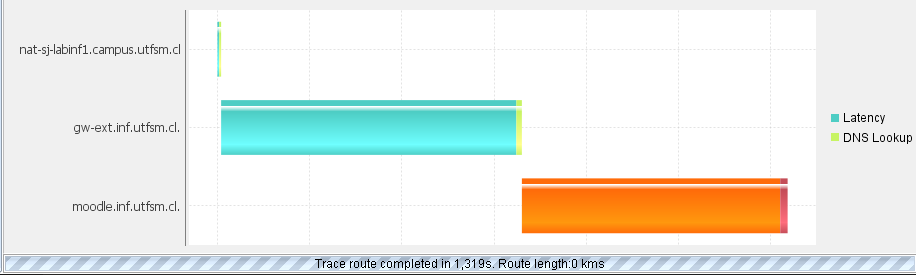
\includegraphics[width=1\textwidth]{imagenes/moodle_grafica.png} \caption{\small \textbf{Tiempos de latencia de paquetes al ingresar a Moodle.}} 
\label{fig:diagrama_1} 
\end{figure}

\subsubsection{Google}
La tabla y gráficas siguientes corresponden a \emph{http://google.com/}:\\

\begin{table}[H]
\centering
\begin{tabular}{| c | c | c | c | c | c |}
\hline
\# & País & Localidad & Latitud & Longitud & IP\\
\hline
1 & Chile & Valparaiso & -33.047806 & -71.6011 & 200.1.20.155\\
\hline
2 & United States & Chicago & 41.884903 & -87.6238 & 192.169.2.1\\
\hline
3 & United States & Chicago & 41.884903 & -87.6238 & 192.169.3.2\\
\hline
4 & Chile & Valparaiso & -33.047806 & -71.6011 & 200.1.21.131\\
\hline
5 & Chile & Valparaiso & -33.047806 & -71.6011 & 200.1.20.131\\
\hline
6 & Chile & Santiago & -33.449997 & -70.6667 & 190.208.0.173\\
\hline
7 & Chile & Santiago & -33.449997 & -70.6667 & 190.208.5.57\\
\hline
8 & Chile & Santiago & -33.449997 & -70.6667 & 200.27.5.186\\
\hline
9 & Chile & Santiago & -33.449997 & -70.6667 & 190.208.5.86\\
\hline
10 & Chile & Santiago & -33.449997 & -70.6667 & 190.208.9.13\\
\hline
11 & Chile & Santiago & -33.449997 & -70.6667 & 190.208.9.26\\
\hline
12 & United States & Mountain View & 37.419205 & -122.0574 & 72.14.234.41\\
\hline
13 & United States & Mountain View & 37.419205 & -122.0574 & 173.194.42.216\\
\hline
\end{tabular}
\caption{\small \textbf{Ruta por los paquetes al consultar la página de Google.}}
\end{table}

\begin{table}[H]
\centering
\begin{tabular}{| c | c | c | c | c |}
\hline
\# & Hostname & Latencia & Búsqueda & Distancia al nodo\\
 &  & (ms) & DNS (ms) & anterior (km)\\
\hline
1 & nat-sj-labinf1.campus.utfsm.cl & 0 & 0 & 0\\
\hline
2 & (None) & 1 & 2 & 8501\\
\hline
3 & (None) & 3 & 2 & 0\\
\hline
4 & fw.usm.cl. & 2 & 7 & 8501\\
\hline
5 & telmex-gw.usm.cl. & 2 & 3 & 0\\
\hline
6 & 190.208.0.173. & 4 & 9 & 97\\
\hline
7 & 190.208.5.57. & 2 & 17 & 0\\
\hline
8 & (None) & 1 & 3 & 0\\
\hline
9 & 190.208.5.86. & 1 & 13 & 0\\
\hline
10 & 190.208.9.13. & 1 & 2 & 0\\
\hline
11 & 190.208.9.26. & 1 & 2 & 0\\
\hline
12 & (None) & 9 & 153 & 9517\\
\hline
13 &  scl03s05-in-f24.1e100.net. & 2 & 3 & 0\\
\hline
\end{tabular}
\caption{\small \textbf{Continuación de la tabla anterior.}}
\end{table}

\begin{figure}[H] 
\centering 
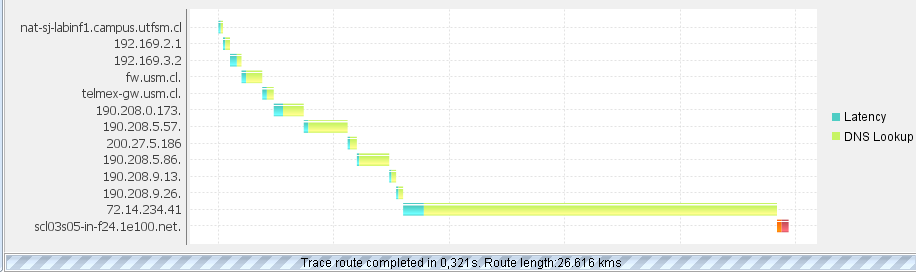
\includegraphics[width=1\textwidth]{imagenes/google_grafica.png} \caption{\small \textbf{Tiempos de latencia de paquetes al ingresar a Google.}} 
\label{fig:diagrama_1} 
\end{figure}

\subsubsection{CIME}
La tabla y gráficas que ahora siguen son las que corresponden al ingreso de \emph{http://cime.cl/}:\\

\begin{table}[H]
\centering
\begin{tabular}{| c | c | c | c | c | c |}
\hline
\# & País & Localidad & Latitud & Longitud & IP\\
\hline
1 & Chile & Valparaiso & -33.047806 & -71.6011 & 200.1.20.155\\
\hline
2 & Chile & Valparaiso & -33.047806 & -71.6011 & 200.1.21.131\\
\hline
3 & Chile & Valparaiso & -33.047806 & -71.6011 & 200.1.20.155\\
\hline
4 & Chile & Santiago & -33.449997 & -70.6667 & 190.208.0.173\\
\hline
5 & Chile & Santiago & -33.449997 & -70.6667 & 190.208.5.77\\
\hline
6 & Chile & Santiago & -33.449997 & -70.6667 & 200.27.5.178\\
\hline
7 & Chile & Santiago & -33.449997 & -70.6667 & 200.27.5.114\\
\hline
8 & Chile & Santiago & -33.449997 & -70.6667 & 190.208.9.9\\
\hline
9 & Chile & Santiago & -33.449997 & -70.6667 & 190.208.9.6\\
\hline
10 & United States & Englewood & 39.623703 & -104.8738 & 129.250.2.110\\
\hline
11 & United States & Englewood & 39.623703 & -104.8738 & 129.250.2.99\\
\hline
12 & United States & Englewood & 39.623703 & -104.8738 & 129.250.4.4\\
\hline
13 & United States & New York & 40.7267 & -73.9981 & 192.241.164.238\\
\hline
14 & United States & New York & 40.7267 & -73.9981 & 107.170.72.180\\
\hline
\end{tabular}
\caption{\small \textbf{Ruta por los paquetes al consultar la página de CIME.}}
\end{table}

\begin{table}[H]
\centering
\begin{tabular}{| c | c | c | c | c |}
\hline
\# & Hostname & Latencia & Búsqueda & Distancia al nodo\\
 &  & (ms) & DNS (ms) & anterior (km)\\
\hline
1 & nat-sj-labinf1.campus.utfsm.cl & 0 & 0 & 0\\
\hline
2 & fw.usm.cl. & 37 & 3 & 0\\
\hline
3 & telmex-gw.usm.cl. & 27 & 3 & 0\\
\hline
4 & 190.208.0.173. & 1 & 186 & 97\\
\hline
5 & 190.208.5.77. & 0 & 46 & 0\\
\hline
6 & (None) & 1 & 289 & 0\\
\hline
7 & Ge1-2.igr1.Santiago.ip.telmexchile.cl. & 59 & 84 & 0\\
\hline
8 & 190.208.9.9. & 36 & 62 & 0\\
\hline
9 & 190.208.9.6. & 36 & 27 & 0\\
\hline
10 & ae-3.r20.miamifl02.us.bb.gin.ntt.net. & 1 & 4 & 8864\\
\hline
11 & ae-8.r21.asbnva02.us.bb.gin.ntt.net. & 10 & 3 & 0\\
\hline
12 & ae-8.r20.asbnva02.us.bb.gin.ntt.net. & 46 & 4 & 0\\
\hline
13 & (None) & 34 & 10507 & 2615\\
\hline
14 & (None) & 1 & 369 & 0\\
\hline
\end{tabular}
\caption{\small \textbf{Continuación de la tabla anterior.}}
\end{table}

\begin{figure}[H] 
\centering 
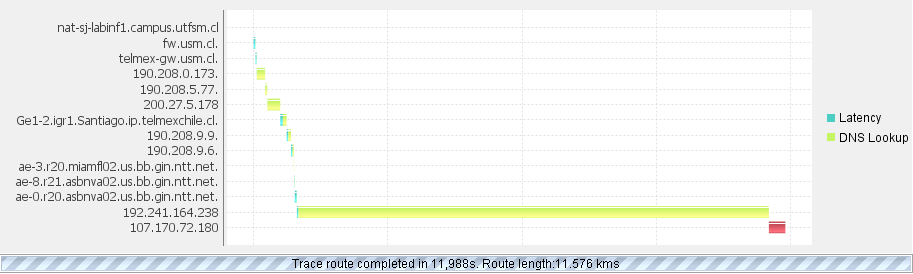
\includegraphics[width=1\textwidth]{imagenes/cime_grafica.png} \caption{\small \textbf{Tiempos de latencia de paquetes al ingresar a CIME.}}
\label{fig:diagrama_1} 
\end{figure}

\subsubsection{Wikipedia}
Las tablas y gráfica para el ingreso a \emph{http://wikipedia.com/} son las siguientes:\\

\begin{table}[H]
\centering
\begin{tabular}{| c | c | c | c | c | c |}
\hline
\# & País & Localidad & Latitud & Longitud & IP\\
\hline
1 & Chile & Valparaiso & -33.047806 & -71.6011 & 200.1.20.155\\
\hline
2 & Chile & Valparaiso & -33.047806 & -71.6011 & 200.1.21.131\\
\hline
3 & Chile & Valparaiso & -33.047806 & -71.6011 & 200.1.20.131\\
\hline
4 & Chile & Santiago & -33.449997 & -70.6667 & 190.208.0.173\\
\hline
5 & Chile & Santiago & -33.449997 & -70.6667 & 190.208.5.77\\
\hline
6 & Chile & Santiago & -33.449997 & -70.6667 & 200.27.5.178\\
\hline
7 & Chile & Santiago & -33.449997 & -70.6667 & 200.27.5.206\\
\hline
8 & Chile & Santiago & -33.449997 & -70.6667 & 190.208.9.9\\
\hline
9 & Chile & Santiago & -33.449997 & -70.6667 & 190.208.9.6\\
\hline
10 & United States & Englewood & 39.623703 & -104.8738 & 157.238.179.17\\
\hline
11 & United States & Englewood & 39.623703 & -104.8738 & 129.250.2.184\\
\hline
12 & United States & Englewood & 39.623703 & -104.8738 & 129.250.4.207\\
\hline
13 & United States & Englewood & 39.623703 & -104.8738 & 129.250.204.190\\
\hline
14 & United States & San Francisco & 37.789795 & -122.394196 & 208.80.154.224\\
\hline
\end{tabular}
\caption{\small \textbf{Ruta por los paquetes al consultar la página de Wikipedia.}}
\end{table}

\begin{table}[H]
\centering
\begin{tabular}{| c | c | c | c | c |}
\hline
\# & Hostname & Latencia & Búsqueda & Distancia al nodo\\
 &  & (ms) & DNS (ms) & anterior (km)\\
\hline
1 & nat-sj-labinf1.campus.utfsm.cl & 0 & 0 & 0\\
\hline
2 & fw.usm.cl. & 1 & 11 & 0\\
\hline
3 & telmex-gw.usm.cl. & 1 & 3 & 0\\
\hline
4 & 190.208.0.173. & 7 & 5 & 97\\
\hline
5 & 190.208.5.77. & 2 & 4 & 0\\
\hline
6 & (None) & 8 & 2 & 0\\
\hline
7 & (None) & 105 & 16 & 0\\
\hline
8 & 190.208.9.9. & 2 & 5 & 0\\
\hline
9 & 190.208.9.6. & 1 & 11 & 0\\
\hline
10 & xe-0-4-0-2.r05.miamfl02.us.bb.gin.ntt.net. & 69 & 6 & 8864\\
\hline
11 & ae-4.r20.miamfl02.us.bb.gin.ntt.net. & 25 & 3 & 0\\
\hline
12 & ae-2.r04.asbnva02.us.bb.gin.ntt.net. & 140 & 22 & 0\\
\hline
13 & xe-0-7-0-8.r04.asbnva02.us.ce.gin.ntt.net. & 69 & 3 & 0\\
\hline
14 & text-lb.eqiad.wikimedia.org. & 78 & 1584 & 1533\\
\hline
\end{tabular}
\caption{\small \textbf{Continuación de la tabla anterior.}}
\end{table}

\begin{figure}[H] 
\centering 
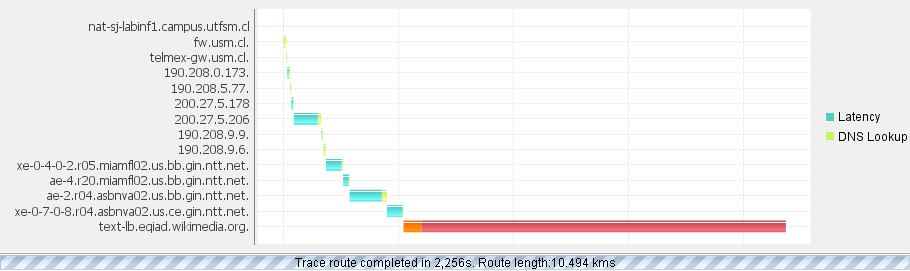
\includegraphics[width=1\textwidth]{imagenes/wiki_grafica.png} \caption{\small \textbf{Tiempos de latencia de paquetes al ingresar a Wikipedia.}}
\label{fig:diagrama_1} 
\end{figure}

\subsubsection{Embajada de Australia en Chile}
Al ingresar a \emph{http://www.chile.embassy.gov.au/} se obtuvieron las siguientes tablas y gráfica que representa latencias. Cabe destacar que para el traceroute realizado a este sitio web, al llegar al router situado en Japón, OVT se quedó colgado, así que la ejecución terminó en ese punto.\\

\begin{table}[H]
\centering
\begin{tabular}{| c | c | c | c | c | c |}
\hline
\# & País & Localidad & Latitud & Longitud & IP\\
\hline
1 & Chile & Valparaiso & -33.047806 & -71.6011 & 200.1.20.155\\
\hline
2 & United States & Chicago & 41.884903 & -87.6238 & 192.169.2.1\\
\hline
3 & United States & Chicago & 41.884903 & -87.6238 & 192.169.3.2\\
\hline
4 & Chile & Valparaiso & -33.047806 & -71.6011 & 200.1.21.131\\
\hline
5 & Chile & Valparaiso & -33.047806 & -71.6011 & 200.1.20.131\\
\hline
6 & Chile & Santiago & -33.449997 & -70.6667 & 190.208.0.173\\
\hline
7 & Chile & Santiago & -33.449997 & -70.6667 & 190.208.5.53\\
\hline
8 & Chile & Santiago & -33.449997 & -70.6667 & 200.27.5.178\\
\hline
9 & Chile & Santiago & -33.449997 & -70.6667 & 200.27.5.114\\
\hline
10 & Chile & Santiago & -33.449997 & -70.6667 & 190.208.9.9\\
\hline
11 & Chile & Santiago & -33.449997 & -70.6667 & 190.208.9.86\\
\hline
12 & United States & New York & 40.758804 & -73.968 & 173.241.129.209\\
\hline
13 & France & (Unknown) & 48.86 & 2.350006 & 77.67.68.234\\
\hline
14 & France & (Unknown) & 48.86 & 2.350006 & 141.136.105.34\\
\hline
15 & Japan & (Unknown) & 35.690002 & 139.69 & 202.147.50.186\\
\hline
16 & Asia/Pacific Region & (Unknown) & 35.0 & 105.0 & 203.192.174.137\\
\hline
17 & Asia/Pacific Region & (Unknown) & 35.0 & 105.0 & 203.192.174.165\\
\hline
18 & Japan & (Unknown) & 35.690002 & 139.69 & 202.147.42.160\\
\hline
\end{tabular}
\caption{\small \textbf{Ruta por los paquetes al consultar la página de la embajada de Australia en Chile.}}
\end{table}

\begin{table}[H]
\centering
\begin{tabular}{| c | c | c | c | c |}
\hline
\# & Hostname & Latencia & Búsqueda & Distancia al nodo\\
 &  & (ms) & DNS (ms) & anterior (km)\\
\hline
1 & nat-sj-labinf1.campus.utfsm.cl & 0 & 0 & 0\\
\hline
2 & (None) & 2 & 7 & 8501\\
\hline
3 & (None) & 3 & 2 & 0\\
\hline
4 & fw.usm.cl. & 42 & 30 & 8501\\
\hline
5 & telmex-gw.usm.cl. & 2 & 5 & 0\\
\hline
6 & 190.208.0.173. & 41 & 3 & 97\\
\hline
7 & 190.208.5.53. & 1 & 4 & 0\\
\hline
8 & (None) & 7 & 7 & 0\\
\hline
9 & Ge1-2.igr1.Santiago.ip.telmexchile.cl. & 25 & 2 & 0\\
\hline
10 & 190.208.9.9. & 0 & 3 & 0\\
\hline
11 & 190.208.9.86. & 1 & 3 & 0\\
\hline
12 & ae2-202.nyc20.ip4.tinet.net. & 140 & 5 & 8267\\
\hline
13 & pacnet-gw.ip4.tinet.net. & 56 & 4 & 5837\\
\hline
14 & (None) & 10 & 12 & 0\\
\hline
15 & be1.gw4.sjc1.asianetcom.net. & 12 & 3 & 9722\\
\hline
16 & te0-1-0-0-981.cr2.syd5.asianetcom.net. & 151 & 22 & 3134\\
\hline
17 & te0-0-0-0.cr1.syd5.asianetcom.net. & 1 & 8 & 0\\
\hline
18 & ge-2-1-0-0.gw1.cbr1.asianetcom.net. & 129 & 4 & 3134\\
\hline
\end{tabular}
\caption{\small \textbf{Continuación de la tabla anterior.}}
\end{table}

\begin{figure}[H] 
\centering 
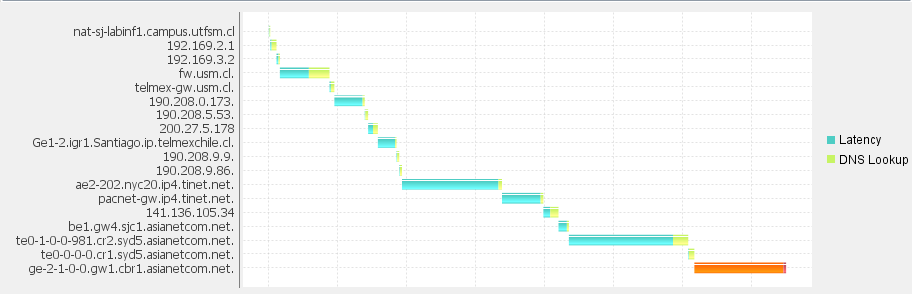
\includegraphics[width=1\textwidth]{imagenes/australia_grafica_sinfin.png} \caption{\small \textbf{Tiempos de latencia de paquetes al ingresar al sitio de la embajada de Australia en Chile.}}
\label{fig:diagrama_1} 
\end{figure}

\subsubsection{Conclusiones y respuestas}
\textbf{\textit{¿Por qué los paquetes toman las rutas descritas en el programa OVT?}} Los paquetes son direccionados por los routers de acuerdo a la información que manejan en sus tablas de ruteo. Hay que destacar que cada router no necesita saber la ruta completa para los paquetes en cuestión, sino que sólo les basta determinar el siguiente salto y por qué puerta de enlace deben enviarse los paquetes.\\

El hecho de que para cada ocasión que se haga un traceroute se puedan obtener rutas ligeramente distintas, depende en primer lugar de la posición geográfica desde donde se efectúa la petición del sitio web, y el protocolo IP es quien determina cuál sería la mejor ruta para los saltos, adaptándose en todo momento a las condiciones de la red. Esto último quiere decir que las tablas de ruteo van cambiando con el tiempo.\\

La ruta se va generando, esto es, el traceroute basa su funcionamiento en el uso del campo TTL (Time To Live) que contienen los datagramas IP. El TTL indica la cantidad de routers por los cuales el datagrama va a circular antes de que se le de por descartado. Colgándose de eso, traceroute lo que realiza es enviar los paquetes con TTL incrementales, partiendo desde TTL = 1. Siguiendo esa lógica, el primer paquete será descartado (el router al que llegó le decrementará su TTL a cero, por lo tanto se descarta), y entonces, el router que le ha desechado enviará de vuelta un mensaje ICMP "TTL Expired", que dentro de sí tiene el nombre del router al que llegó el paquete y su IP. Luego de ello, el emisor de los paquetes vuelve a enviar, pero con un TTL = 2, consiguiendo que el paquete pase no por un router, sino que por dos, y el segundo router hará lo mismo que hizo el primero cuando el paquete que se envió tenía TTL = 1. Después de toda la sucesión de pasos descritos, se puede ir completando la ruta con los datos obtenidos, y al llegar al router de destino, éste envía un mensaje ICMP "Dest port unreachable", y así el traceroute termina.\\

\textbf{\textit{Y entonces, ¿cómo es que viajan los paquetes entre continentes?}} Usando la técnica anterior relacionada con los tiempos de vida, y también gracias a la fragmentación y reensamblaje (IPv4), los paquetes pueden ir viajando desde las redes más pequeñas y con menor calidad de tráfico, hasta redes mundiales de grandes prestaciones. Gracias a lo anterior, todo este viaje a través de la gran red de redes puede abrirse paso a través de los continentes por medio de las diversas tecnologías de comunicación que incluyen conexiones básicas como las telefónicas o inalámbricas caseras, pasando por conexiones 3G/4G, hasta enlaces físicos de mayor rendimientos como los cableados, de fibra óptica y satelitales, siendo enlaces como los últimos descritos los que se sitúan entre continentes.\\

\textbf{\textit{Los enlaces internacionales de Chile}}, siguiendo la lógica de que corresponden a \emph{la dirección IP del último router situado en Chile antes de que se pase a uno del extranjero}, según los resultados obtenidos usando OVT, son los siguientes:

\begin{table}[H]
\centering
\begin{tabular}{| c | c | c | c | c |}
\hline
Localidad & Latitud & Longitud & IP & Hostname\\
\hline
Santiago & -33.449997 & -70.6667 & 190.208.9.86 & 190.208.9.86.\\
\hline
Santiago & -33.449997 & -70.6667 & 190.208.9.6 & 190.208.9.6.\\
\hline
Santiago & -33.449997 & -70.6667 & 190.208.9.26 & 190.208.9.26.\\
\hline
\end{tabular}
\caption{\small \textbf{Enlaces internacionales de Chile.}}
\end{table}

Hay que destacar que en el caso de la embajada de Australia y Google para el enlace:

\begin{table}[H]
\centering
\begin{tabular}{ c  c  c  c  c }
Localidad & Latitud & Longitud & IP & Hostname\\
Valparaíso & -33.047806 & -71.6011 & 200.1.20.155 & nat-sj-labinf1.campus.utfsm.cl\\
\end{tabular}
\end{table}

que corresponde al router asociado a la red ''di'' de la universidad, hace un salto directo hacia el extranjero, no así para las otras páginas.

\newpage

\subsection{Aplicación del Algoritmo de Vector-Distancia}

\end{document}